\chapter{Auswertung}
\label{chap:auswertung}
In diesem Kapitel soll die Software anhand von für die Softwareentwicklung relevanten Qualitätsmerkmalen
ausgewertet werden. Laut Peter Liggesmeyer, dem Autor des Buches "Software-Qualität", sind diese
Korrektheit, Vollständigkeit, Sicherheit, Zuverlässigkeit, Verfügbarkeit und Robustheit \cite[S. 5]{SoftwareQualitaet}.

\section{Korrektheit}
\label{sec:korrektheit}
Um die Korrektheit der Gesamtanwendung beurteilen zu können, muss das in der Anforderungsanalyse erwartete
Verhalten mit dem Verhalten des Istzustands verglichen werden. In der Anforderungsanalyse
in \Cref{chap:anforderungsanalyse} wurden allerdings hauptsächlich Funktionalitäten und weniger deren 
Verhalten behandelt. Da das Vorhalten der Software vor der Entwicklung des Konzepts nicht klar definiert wurde,
ist es schwer, die Korrektheit der Anwendung zu beurteilen. Die in der Konzept-Phase erarbeiteten Verfahren
wurden wie in dem Konzept entworfen auch in der Software schlussendlich umgesetzt. So wurden für
das Diagrammanordnungsverfahren ein vielfaches an Modultests implementiert, um das gewollte Verhalten auch in
der Anwendung sicherzustellen. Das in den Konzepten erarbeitete Verhalten weicht nicht von dem der späteren
Umsetzung ab. Dies ist auch für die Schritte des Datenstroms und den angeforderten Funktionalitäten der Fall.
Daraus ist zu schlussfolgern, dass die Software korrekt ist.

\section{Vollstandigkeit}
\label{sec:vollstaendigkeit}
Die Vollständigkeit der Software lässt sich einfach beurteilen. Hierfür müssen nur die in der Anforderungsanalyse
erarbeiteten Funktionalitäten mit denen des Istzustands verglichen werden. Die wichtigsten Funktionalitäten
wurden alle umgesetzt. So kann die Gesamtanwendung Daten beschaffen, verarbeiten, Diagrammen zuweisen und darstellen.
Da sich die Arbeit bei der Konzeption und Implementierung der Software auf die Qualitätsmerkmale Sicherheit,
Zuverlässigkeit, Verfügbarkeit und Robustheit fokussiert hat, konnten nicht alle angeforderten Implementierungsdetails
erfüllt werden. Die Authentifizierung, Rechteverwaltung, Sprachauswahl, Suche, Echtzeitübertragung der Daten wurden
voll funktionsfähig umgesetzt. Nicht oder nur bedingt wurde die Offline-Funktionalität, die Benachrichtigung
des Benutzers bei Übertretung eines vordefinierten Schwellwerts sowie die Filterung der Daten in den Diagrammen.
Die Offline-Funktionalität ist aktuell nur für statische Elemente der Anwendung gegeben. Die über das WebSocket-Protokoll
übertragenen Daten werden aktuell nicht in der progressiven Webanwendung gespeichert. Dies ist allerdings aus technischer
Sicht auch nur bedingt möglich, da das Speichervolumen von vom Browser bereitgestellten Speichermöglichkeiten
je nach Browser variiert und gerade auf mobilen Endgeräten oftmals sehr gering ausfällt \cite{HTML5RocksStorage}.
Die Benachrichtigung der Benutzer bei dem Übertreten eines vordefinierten Schwellwerts wurde noch nicht umgesetzt.
Die Funktionalität ist allerdings für die Zukunft geplant. Die Filterung der Daten ist bedingt möglich. So kann 
man mithilfe der von der Arbeit verwendeten Abfragesprache JMESPath, Daten anhand diverser Kriterien filtern.
Des Weiteren bietet die Visualisierungsbibliothek Chart.js bedingt Filtermöglichkeiten an. Ein selektives Filtern
an beispielsweise der Zeit ist allerdings nach aktuellem Stand innerhalb der Diagramme noch nicht umgesetzt worden.
Die Diagramme wurden allerdings so konzipiert, dass das Hinzufügen einer Filterfunktion
kein Problem darstellen sollte.

\section{Sicherheit}
\label{sec:sicherheit}
Auf die Sicherheit der Anwendung wurde besonders geachtet. So wurde wie bereits in der Implementierung erläutert, neben
der JWT-Authentisierung auch eine TwoZwei-Faktor-Authentisierung implementiert. Außerdem wurden in dem Resource Management Service
der Ein- und Ausgangsverkehr in beide Richtungen mithilfe des Koa Joi Routers validiert. Die Anwendung sowie die dafür benötigten
Daten werden über HTTPS als auch WSS ausgeliefert. Nichtsdestotrotz beinhaltet die Gesamtanwendung
noch Schwachstellen, die es zu eliminieren gilt. Die Authentifizierung passiert wie in der Implementierung beschrieben
über einen im HTTP-Header gesetzten JWT. Bei der WebSocket-Verbindung findet die Authentifizierung beim Handshake des
Verbindungsaufbaus statt. Die Verbindung wird somit nicht getrennt, wenn der Token abläuft. Die Frontendanwendung
schließt allerdings bei der Abmeldung eines Benutzers die WebSocket-Verbindung automatisch. Es wäre allerdings dennoch möglich,
dass bei einer erfolgreichen XSS-Attacke, die WebSocket-Verbindung aufrecht gehalten wird, um so Daten zu stehlen.

Ein weiterer Sachverhalt ist die Verwendung des \code{dangerouslySetInnerHTML} Feldes im React Frontend. Zur Verarbeitung
der Daten wird ein Syntax-Highlighter verwendet, um die Ein- und Ausgangsdaten in Form des JSON-Schemas anzuzeigen.
Da dieser allerdings in React zu langsam war, wurde er in nativem JavaScript implementiert und mithilfe des 
\code{dangerouslySetInnerHTML} Feldes in den React Code eingebunden. Im Falle, dass die externe, als Datenquelle
verwendete API, korrupte Daten ausliefert, könnten diese als Einstiegspunkt für eine XSS-Attacke verwendet werden.
Wenn man allerdings die angezeigten Zeilen der Ein- und Ausgangsdaten auf eine moderate Anzahl begrenzt, kann ein
in React geschriebener Syntax-Highlighter verwendet und somit die Schwachstelle umgangen werden. Die Arbeit plant
für die Zukunft, das JSON-Schema nie ganz anzuzeigen. Ziel ist es, das Schema stückchenweise aufzuklappen.

Der letzte Sicherheitsaspekt, den es anzusprechen gilt, ist die SSH-Verbindung aus der Pipeline heraus zu den Produktionsservern.
Hat ein Eindringling Zugriff auf die Pipeline, hat er gleichzeitig Zugriff auf alle Produktionsserver. 
Um dies zu vermeiden, können WebHooks verwendet werden. So kann die Pipeline eine Nachricht via WebHook an
den Produktionsserver senden, der daraufhin die Docker-Images mit denen aus der Docker Registry austauscht.

\section{Zuverlässigkeit}
\label{sec:zuverlaessigkeit}
Um die Zuverlässigkeit einer Software zu bestimmen, wird oftmals ein Wert verwendet,
der bestimmt, wie lang die Durchschnittszeit bis zum Ausfall des Systems ist.\cite[S. 9]{SoftwareQualitaet}
Ein Softwaresystem kann viele Ausfallgründe haben. Der wohl einfachste ist eine zu hohe Auslastung des Systems.
Dieser Ausfallgrund wird in \Cref{sec:robustheit} genauer betrachtet. Desweiteren kann ein System durch falsche
Eingabewerte oder ein unerwartetes Verhalten eines Nutzers zum Ausfall gebracht werden. Mit automatisierten Langzeittests
sind diese zwei Ausfallgründe allerdings schwer zu berücksichtigen. So müsste der Entwickler bereits bei der Implementierung
der Tests über die möglichen Ausfallgründe bescheid wissen. Um Störfalle zu verhindern, gilt es möglichst viele Szenarien mit
Tests abzudecken. Zur beurteilung der Zuverlässigkeit der Software betrachtet die Arbeit die Testabdeckung der einzelnen Komponenten
des Systems.

Die Arbeit hat sich bei der Implementierung der Tests primär auf Integrationstests fokussiert, um so die fehlerfreie 
Zusammenarbeit der einzelnen Services sicherzustellen. Die Integrationstests gehen gegen die Schnittstellen der Services.
Bei dem Resource Management Service sind alle Routen mit Tests abgedeckt. Für jede Route wurde die Rechteverwaltung,
die Authentisierung, die Validierung der Eingabe und Ausgabewerte sowie die Funktionalität der Route selbst getestet.
Der Data Delivery Service hingegen besitzt zum aktuellen Stand nur rudimentäre Tests der Hauptfunktionalitäten.
Hier wurden nicht wie bei dem Resource Management Service auf falsche Eingabewerte getestet. Außerdem fehlen die für
die Gesamtanwendung wichtigen End-To-End-Tests. Betrachtet man die progressive Webanwendung, wurden dort nur komplexe
Funktionalitäten mit Modultests abgedeckt.

\section{Verfügbarkeit}
\label{sec:verfuegbarkeit}
Die Verfügbarkeit der Anwendung ist sehr hoch. Um die Funktionalität der Lastenverteilung
zu testen, wird in der Frontendanwendung im Administrationsbereich die lokale Netzwerk-IP
der aktuell verwendeten Instanz angezeit. Bei dem Neuladen der Anwendung, rotiert diese
durch alle Instanzen der Services. Der Lastverteiler funktioniert somit einwandfrei.
Überdies wird der Verkehr im Fall eines Ausfalls einer Instanz auf eine gesunde
Instanz verlegt.

\section{Robustheit}
\label{sec:robustheit}
Um die Robustheit der Gesamtanwendung zu testen, führt die Arbeit zwei verschiedene
Arten von Lasttests durch. Zum einen soll das Cluster auf maximale Auslastung getestet
werden. Da eine große Anzahl an Anfragen versendet werden müssen,
wird hierfür der Lasttestdienst Loader.io\footnote{https://loader.io/} verwendet.
Bei den Anfragen handelt es sich um HTTPS-Anfragen, die gegen
die 37KB große \code{index.html} der Frontendanwendung gehen.
Als zweites wird ein Lasttest über zehn Minuten mithilfe der Open Source Software
JMeter\footnote{https://jmeter.apache.org/} durchgeführt. Hier werden mehrere HTTPS- sowie
WSS-Anfrage hintereinander ausgeführt, um das anfängliche Verhalten eines möglichen Benutzers nachzuahmen.
Für den Test wurden fünf Server zu einem Cluster zusammengefügt. Die einzelnen Services wurden
auf zehn Instanzen skaliert.

\begin{table}[h]
\begin{center}
\begin{tabular}{rrrrr}
Anfragen/Sek. & Fehlerrate & min. & max. & durchschn. \\
\hline
100 &  0\% & 86ms & 419ms & 92ms \\
250 &  0\% & 85ms & 549ms & 93ms \\
500 &  0\% & 85ms & 907ms & 95ms \\
1.000 &  0\% & 85ms & 8.431ms & 267ms \\
2.500 &  1,2\% & 90ms & 15.858ms & 1.974ms \\
5.000 &  8,9\% & 86ms & 19.994ms & 3.726ms \\
\end{tabular}
\end{center}
\caption{Antwortzeiten der Lasttests mit Loader.io (1 Minute Laufzeit)}
\label{tab:resultatdeslasttestsmitloaderio}
\end{table}

In Tabelle \ref{tab:resultatdeslasttestsmitloaderio} sieht man die Resultate
der Lasttests mit Loader.io. Es wurden sechs Iterationen durchgeführt.
Die Felder "min.", "max." und "durchschn." beziehen sich auf die minimale,
maximale und durchschnittliche Antwortzeit, die die Server benötigen, um die
Anfragen zu verarbeiten. Für die Lasttests wurden die HTTPS-Anfragen,
die pro Sekunde abgesendet werden, von initial 100 auf bis zu 5.000 erhöht.
Ab ca. 2.500 Anfragen pro Sekunde fängt das Cluster an, Antworten auf die
Anfragen erst so spät zu versenden, dass die Antwort, die vom Client
erwartete Maximalzeit überschreitet. Betrachtet man die maximale Antwortzeit,
kann man erkennen, dass das Gesamtsystem bereits ab hundert Anfragen pro Sekunde
überlastet ist. Ein Nutzer sollte keine acht Sekunden auf eine Antwort warten
müssen.

\begin{figure}
    \begin{center}
    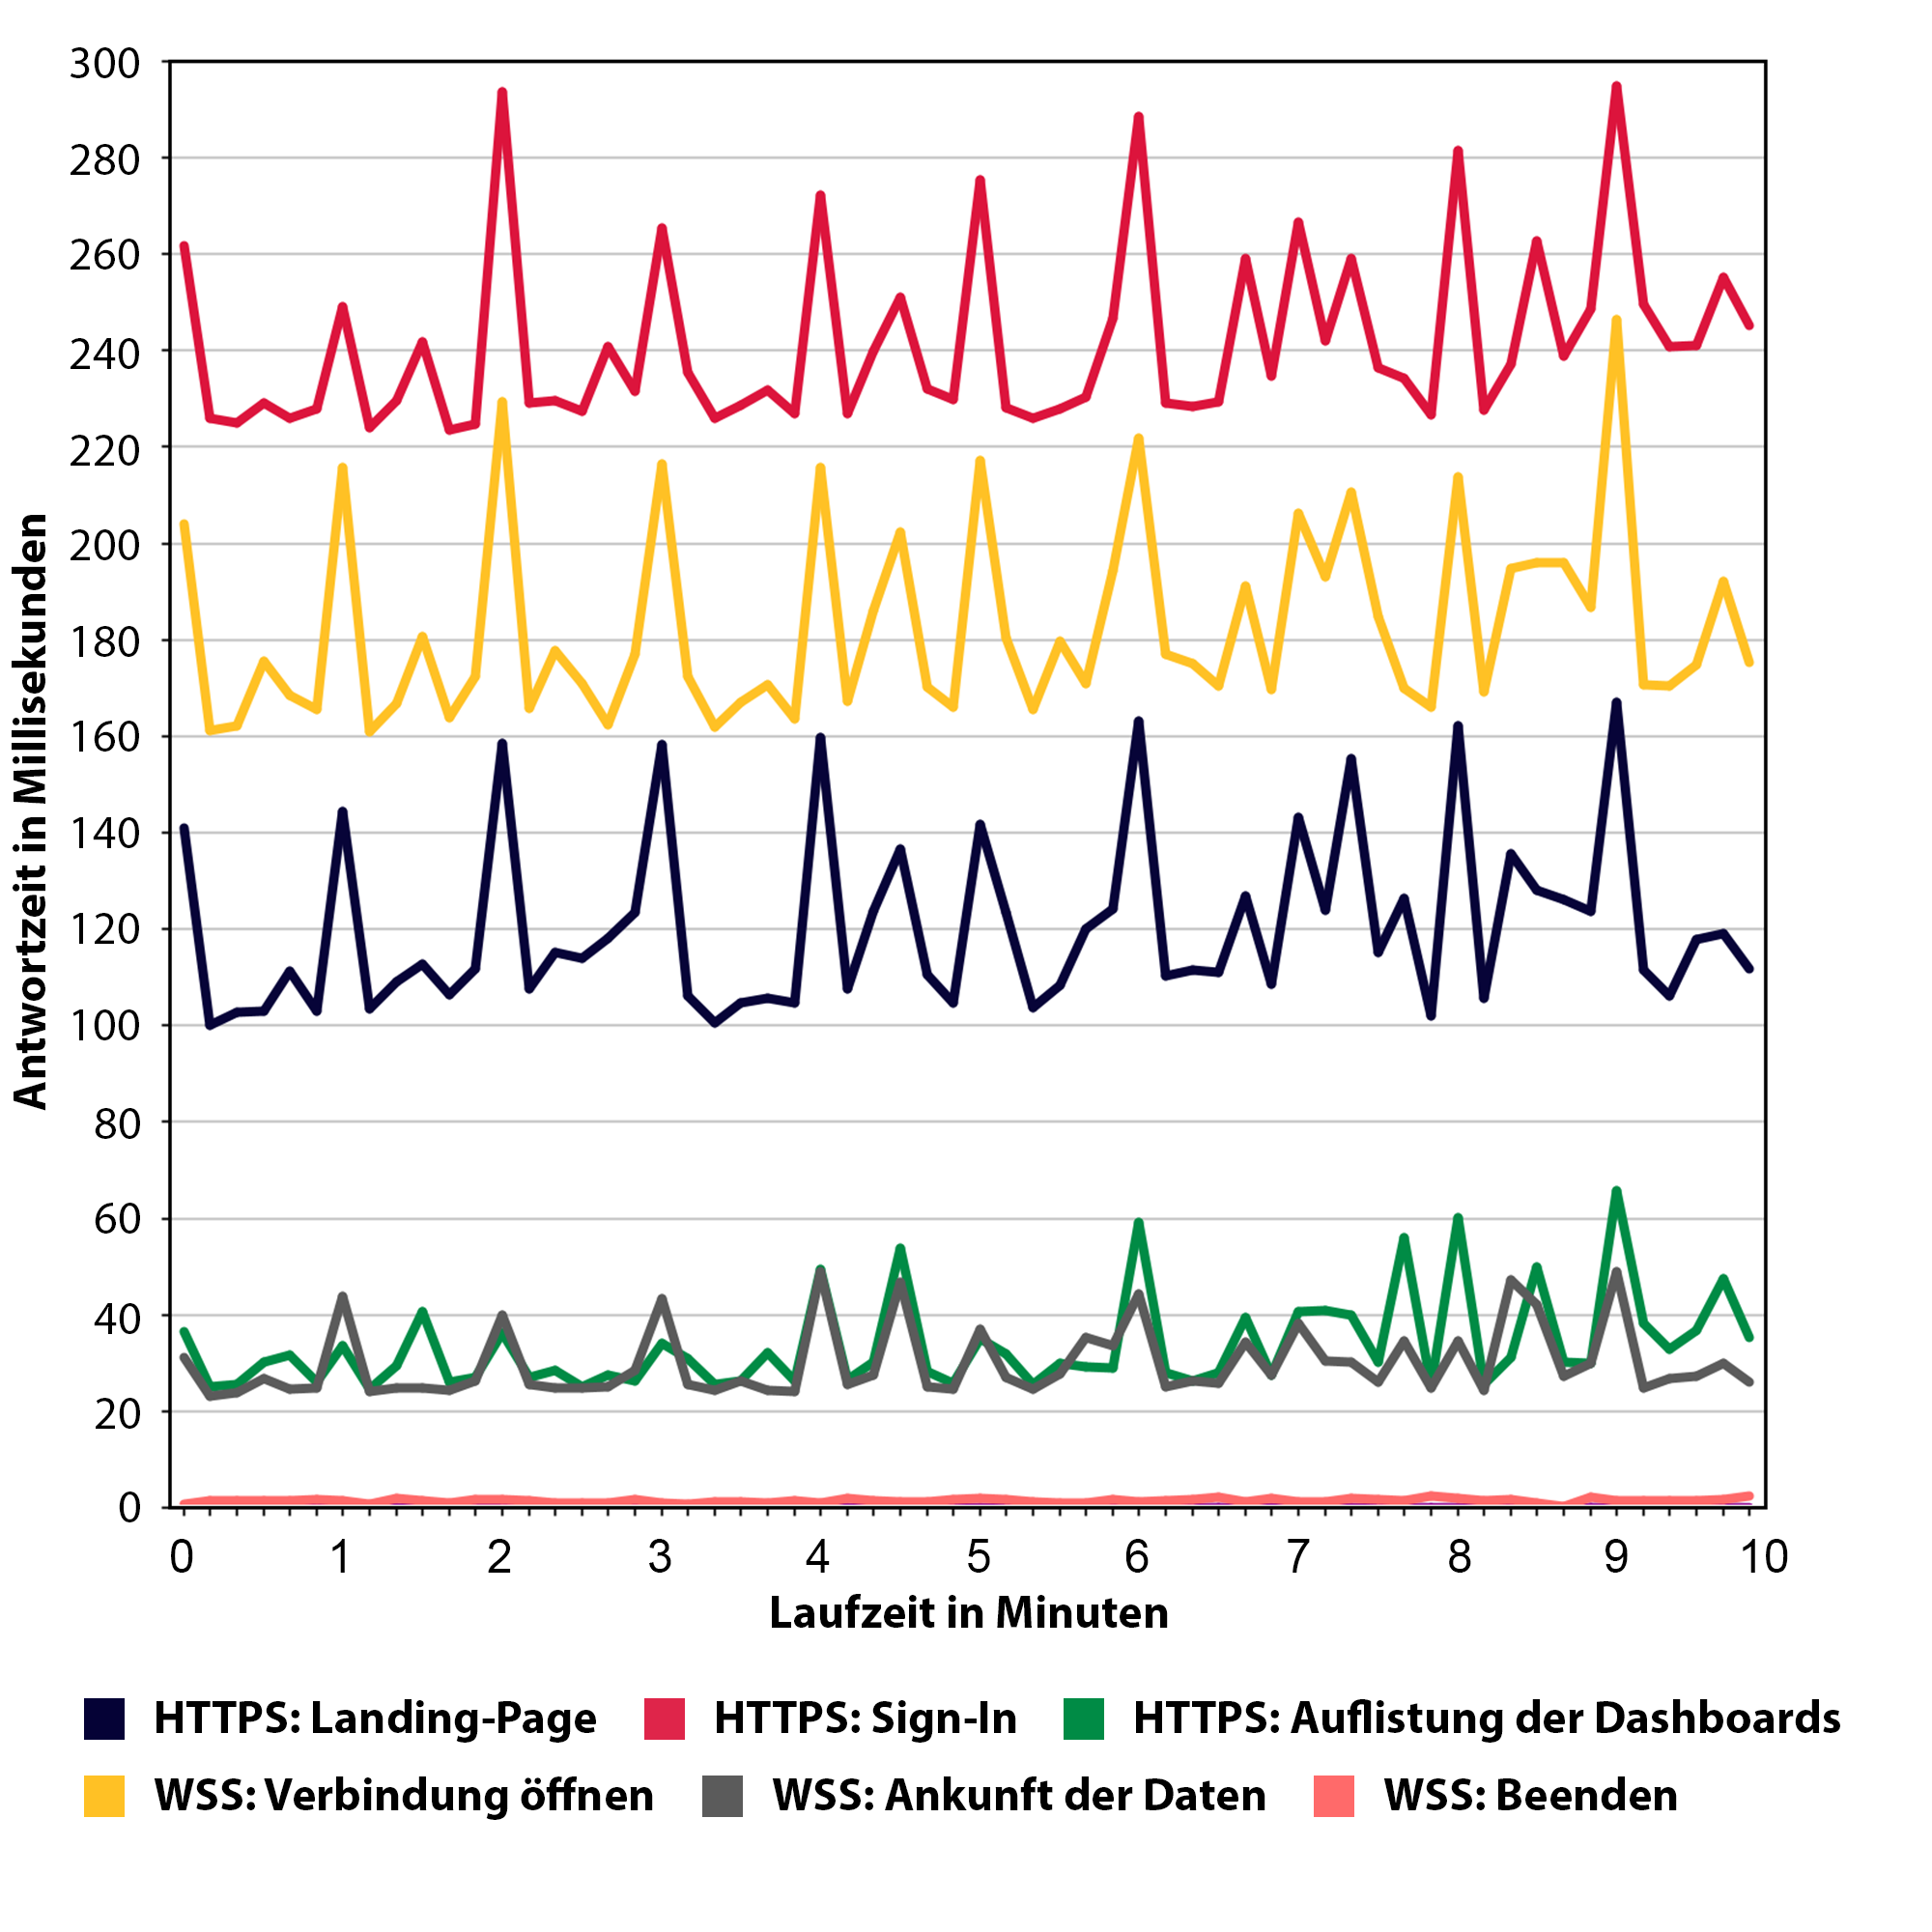
\includegraphics[scale=0.125]{img/abbildungen/Antwortzeitdiagramm}
    \end{center}
    \caption{Lasttest mit JMeter}
    \label{figure:lasttestmitjmeter}
\end{figure}

Die Lasttestresultate der JMeter-Tests sind auf der Abbildung \ref{figure:lasttestmitjmeter}
zu erkennen. Das Diagramm zeigt die Anzahl der jeweils empfangenen Statuscodes in Bezug
auf die verstrichene Zeit. Der Lasttest wurde nach ca. 10 Minuten abgebrochen.
Der Test führt folgendes Szenario zehn mal in der Sekunde aus:
Als erstes wird eine HTTPS-Anfrage an die \code{index.html} gesendet.
Daraufhin loggt sich der Benutzer mit seinen Benutzerdaten ein.
Sobald er eingeloggt ist, läd der Benutzer über die Resource Management Service
eine Liste der Dashboards. Als nächstes wird eine WebSocket-Verbindung eröffnet
und auf eine Datenquelle abonniert. Nach Ankunft der ersten Daten der
Datenquelle wird die WebSocket-Verbindung wieder geschlossen.

Im Schaubild ist zu erkennen, dass das Cluster alle ca. 50 Sekunden einen Einbruch
der Leistung ausweist. Womöglich passiert dies durch einen von Docker Swarm ausgeführten
Cron-Jobs. Interessant ist, dass die Log-In-Anfrage die längste Antwortzeit besitzt.
Bei der Anmeldung wird das Password gegen den Passwort-Hash in der Datenbank verglichen,
ein JWT generiert und als Cookie im Browser gesetzt. Das Aufbauen der WebSocket-Verbindung
braucht am zweitlängsten. Das Laden der Landing-Page liegt im Durchschnitt. Die Anfrage gegen
die Liste der Dashboards sowie der Datentransfer der Beispieldaten über die WebSocket-Verbindung
sind sehr performant.

Die Lasttests bestätigen, dass eine solide Robustheit der Gesamtanwendung gegeben ist. Nichtsdestotrotz
können einzelne Anfragen wie beispielsweise die Login-Route verbessert werden, um die Leistung
der Gesamtanwendung zu steigern. Wie viele Benutzer ein solches Cluster mit fünf Servereinheiten
bedienen kann, ist schwer einzuschätzen. Zum einen verteilt sich die Hauptlast je nach
Benutzergruppe über mehrere Stunden am Tag. Zum anderen sind die in der Arbeit ausgeführten
Lasttests nur schwer mit dem Verhalten echter Nutzer vergleichbar.
